
\documentclass{beamer}
\usetheme{ucl}

\usepackage[utf8]{inputenc}


%%% Increase the height of the banner: the argument is a scale factor >=1.0
%\setbeamertemplate{banner}[ucl][10.0]

%%% Change the colour of the main banner
%%% The background should be one of the UCL colours (except pink or white):
%%%   black,darkpurple,darkred,darkblue,darkgreen,darkbrown,richred,midred,
%%%   navyblue,midgreen,darkgrey,orange,brightblue,brightgreen,lightgrey,
%%%   lightpurple,yellow,lightblue,lightgreen,stone
\setbeamercolor{banner}{bg=darkpurple}
%\setbeamercolor{banner}{bg=yellow,fg=black}

%%% Add a stripe behind the banner
%\setbeamercolor{banner stripe}{bg=darkpurple,fg=black}

%%% The main structural elements
\setbeamercolor{structure}{fg=black}

%%% Author/Title/Date and slide number in the footline
\setbeamertemplate{footline}[author title date]

%%% Puts the section/subsection in the headline
% \setbeamertemplate{headline}[section]

%%% Puts a navigation bar on top of the banner
%%% For this to work correctly, the each \section command needs to be
%%% followed by a \subsection. Requires one extra compile.
% \setbeamertemplate{headline}[miniframes]
%%% Accepts an optional argument determining the width
% \setbeamertemplate{headline}[miniframes][0.3\paperwidth]


%%% Puts the frame title in the banner
%%% Won't work correctly with the above headline templates
%\useoutertheme{ucltitlebanner}
%%% Similar to above, but smaller (and puts subtitle on same line as title)
\useoutertheme[small]{ucltitlebanner}

%%% Gives block elements (theorems, examples) a border
% \useinnertheme{blockborder}
%%% Sets the body of block elements to be clear
% \setbeamercolor{block body}{bg=white,fg=black}

%%% Include CSML logo on title slide
%\titlegraphic{\includegraphics[width=0.16\paperwidth]{csml_logo}}

%%% Include CSML logo in bottom right corner of all slides
%\logo{\includegraphics[width=0.12\paperwidth]{csml_logo}}

%%% Set a background colour
% \setbeamercolor{background canvas}{bg=lightgrey}

%%% Set a background image
%%% Some sample images are available from the UCL image store:
%%%   https://www.imagestore.ucl.ac.uk/home/start
% \setbeamertemplate{background canvas}{%
%   \includegraphics[width=\paperwidth]{imagename}}



%%%%%% Some other settings that can make things look nicer
%%% Set a smaller indent for description environment
\setbeamersize{description width=2em}
%%% Remove nav symbols (and shift any logo down to corner)
\setbeamertemplate{navigation symbols}{\vspace{-2ex}}








\DeclareMathOperator{\Cov}{Cov}
\DeclareMathOperator{\Var}{Var}
\DeclareMathOperator{\E}{\mathbb{E}}
\DeclareMathOperator{\Proba}{\mathbb{P}}

\newcommand{\Covb}[2]{\ensuremath{\Cov\!\left[#1,#2\right]}}
\newcommand{\Eb}[1]{\ensuremath{\E\!\left[#1\right]}}
\newcommand{\Pb}[1]{\ensuremath{\Proba\!\left[#1\right]}}
\newcommand{\Varb}[1]{\ensuremath{\Var\!\left[#1\right]}}

% norm
\newcommand{\norm}[1]{\| #1 \|}

\newcommand{\indep}{\rotatebox[origin=c]{90}{$\models$}}





\usepackage{mathptmx,amsmath,amssymb,graphicx,bibentry,bbm,ragged2e}
\usepackage[english]{babel}

\makeatletter

\newcommand{\noun}[1]{\textsc{#1}}
\newcommand{\jitem}[1]{\item \begin{justify} #1 \end{justify} \vfill{}}
\newcommand{\sframe}[2]{\frame{\frametitle{#1} #2}}

\newenvironment{centercolumns}{\begin{columns}[c]}{\end{columns}}
%\newenvironment{jitem}{\begin{justify}\begin{itemize}}{\end{itemize}\end{justify}}



%\usetheme{Warsaw}
%\setbeamertemplate{footline}[text line]{}
%\setbeamertemplate{headline}{}
%\setbeamercolor{structure}{fg=purple!50!blue, bg=purple!50!blue}

%\setbeamersize{text margin left=15pt,text margin right=15pt}

%\setbeamercovered{transparent}


\@ifundefined{showcaptionsetup}{}{%
 \PassOptionsToPackage{caption=false}{subfig}}
\usepackage{subfig}

\usepackage[utf8]{inputenc}
\usepackage[T1]{fontenc}

\usepackage{multirow}


\makeatother

\def \draft {1}

\usepackage{xparse}
\usepackage{ifthen}
\DeclareDocumentCommand{\comment}{m o o o o}
{\ifthenelse{\draft=1}{
    \textcolor{red}{\textbf{C : }#1}
    \IfValueT{#2}{\textcolor{blue}{\textbf{A1 : }#2}}
    \IfValueT{#3}{\textcolor{ForestGreen}{\textbf{A2 : }#3}}
    \IfValueT{#4}{\textcolor{red!50!blue}{\textbf{A3 : }#4}}
    \IfValueT{#5}{\textcolor{Aquamarine}{\textbf{A4 : }#5}}
 }{}
}
\newcommand{\todo}[1]{
\ifthenelse{\draft=1}{\textcolor{red!50!blue}{\textbf{TODO : \textit{#1}}}}{}
}




\begin{document}

\title{Blockchain, smart cities and territories}
\author{J.~Raimbault$^{1,2,3,4\ast}$\\\medskip
$^{\ast}$\texttt{juste.raimbault@polytechnique.edu}
}

\institute{$^{1}$LASTIG, Univ Gustave Eiffel, IGN-ENSG\\
$^{2}$CASA, University College London\\
$^{3}$UPS CNRS 3611 Complex Systems Institute Paris\\
$^{4}$UMR CNRS 8504 G{\'e}ographie-cit{\'e}s
}


\date{Blockchain pour la valorisation de la recherche\\
ISC-PIF, 13/05/2022
}

\frame{\maketitle}


\sframe{From smart to sustainable cities?}{

% - smart cities and territories, lien avec valo recherche? better governance, management, knowledge transfer
% - theory/governance: Mora, L., Deakin, M., Zhang, X., Batty, M., de Jong, M., Santi, P., & Appio, F. P. (Eds.). (2022). Sustainable Smart City Transitions: Theoretical Foundations, Sociotechnical Assemblage and Governance Mechanisms. Routledge. https://books.google.fr/books?id=uHxTEAAAQBAJ&lpg=PT8&ots=YBm_fAdvpZ&dq=Sustainable%20Smart%20City%20Transitions%3A%20Theoretical%20Foundations%2C%20Sociotechnical%20Assemblage%20and%20Governance%20Mechanisms&lr&hl=fr&pg=PT14#v=onepage&q&f=false

New urban data and smart cities paradigms: applications to urban governance? \cite{mora2022sustainable}

\medskip

$\rightarrow$ \textit{role of blockchain in smart cities technologies and research transfer for sustainable transitions?}

\bigskip

Towards multi-level theories, model and governance for territorial systems \cite{rozenblat2018conclusion}

\medskip

$\rightarrow$ \textit{links between geographical urban theories and urban data science?}

\bigskip

\textbf{Outline:}

\begin{enumerate}
	\item Smart cities and urban analytics
	\item Blockchain for smart cities
	\item Discussion
\end{enumerate}


}



\sframe{Real-time GIS for smart cities}{



% - real-time GIS data Li, W., Batty, M., & Goodchild, M. F. (2020). Real-time GIS for smart cities. International Journal of Geographical Information Science, 34(2), 311-324.

Real-time spatial data monitoring and processing at the core of smart cities approaches \cite{li2020real}

\centering

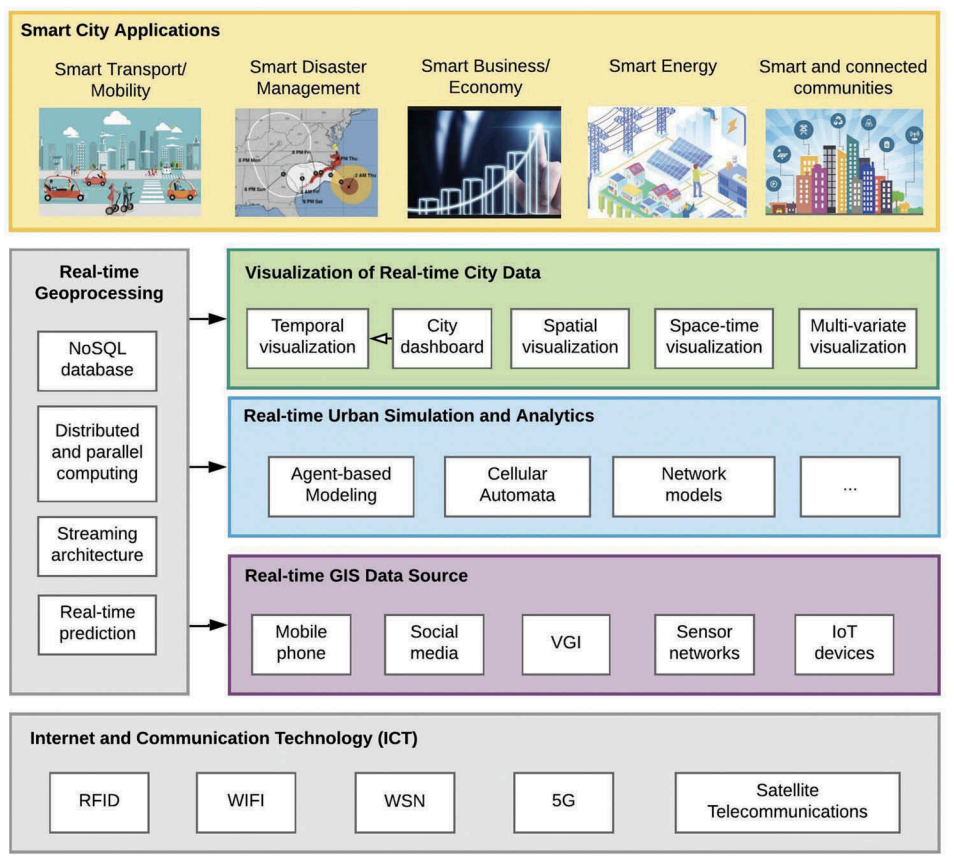
\includegraphics[height=0.8\textheight]{figures/realtimeGIS.png}


}




\sframe{Digital twins}{

% - link model - real system Batty, M. (2019). A map is not the territory, or is it?. Environment and Planning B: Urban Analytics and City Science, 46(4), 599-602.

% - digital twins Batty, M. (2018). Digital twins. Environment and Planning B: Urban Analytics and City Science, 45(5), 817-820.

% - multimodeling Batty, M. (2021). Multiple models. Environment and Planning B: Urban Analytics and City Science, 48(8), 2129-2132.


Concept of \textbf{Digital Twins} underlying several smart cities implementations

\bigskip

$\rightarrow$ hybrid system composed by a technical artefact and a full simulation model of it, coupled in real-time \cite{batty2018digital}

\medskip


$\rightarrow$ fuzzy boundaries and model scope \cite{batty2019map}

\medskip


$\rightarrow$ multi-modeling to capture complementary dimensions \cite{batty2021multiple}

}





\sframe{Definitions of smart cities}{

% - Soe, R. M., Schuch de Azambuja, L., Toiskallio, K., Nieminen, M., & Batty, M. (2021). Institutionalising smart city research and innovation: from fuzzy definitions to real-life experiments. Urban Research & Practice, 1-43.pdf en pj

% more than 8 definitions
% two main models

Research on smart cities and concrete implementations \cite{soe2022institutionalising}

\bigskip

$\rightarrow$ More than 8 definitions with very different scopes: ICT and classical infrastructures, quality of life, sustainability, resilience, empowerment of citizens, \ldots

\medskip

$\rightarrow$ Two main models: top-down planned ``pop-up'' cities (fast urbanising countries such as China) vs integration of ICT in existing infrastructures (Europe and Northern America)


}


\sframe{Critiques of smart cities}{

% a self fulfilling prophecy? A Picon

Antoine Picon, \textit{Smart cities. Théorie et critique d’un idéal auto-réalisateur} \cite{picon2013smart} \cite{rolland2015antoine}

``\textit{How can smart cities come of age?}''

\medskip

% definition? sustainable dev and quality of life? in practice TIC fro better management, adaptation, resilience
% history of technology: empowering and alienating
% role of large companies
% Comment faire vieillir les villes intelligentes?

$\rightarrow$ no clear definition: utopia of sustainability and quality of life - in practice ICT to improve level of service

$\rightarrow$ history of technology: always empowering and alienating

$\rightarrow$ stakeholders: role large digital companies pushing the paradigm?

\bigskip

\centering

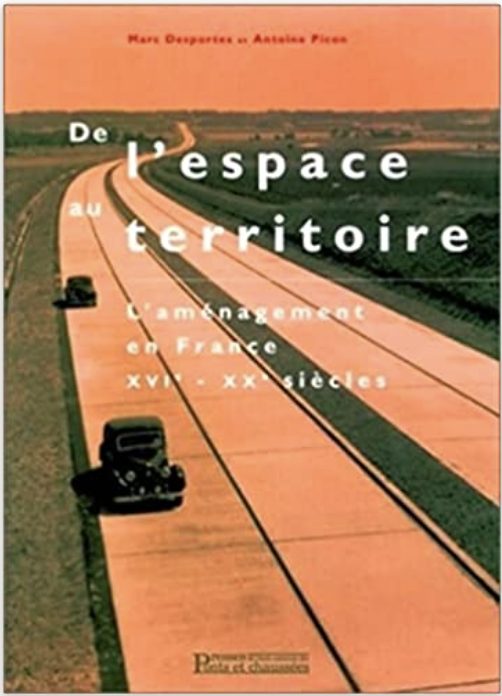
\includegraphics[height=0.4\textheight]{figures/picon_espace.png}\hspace{0.5cm}
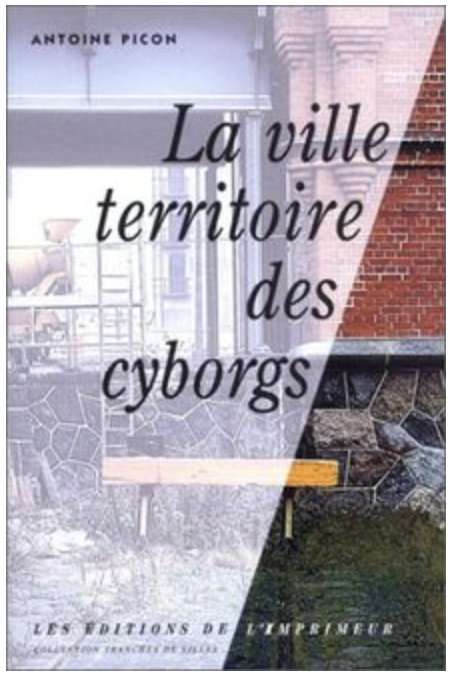
\includegraphics[height=0.4\textheight]{figures/picon_cyborgs.png}\hspace{0.5cm}
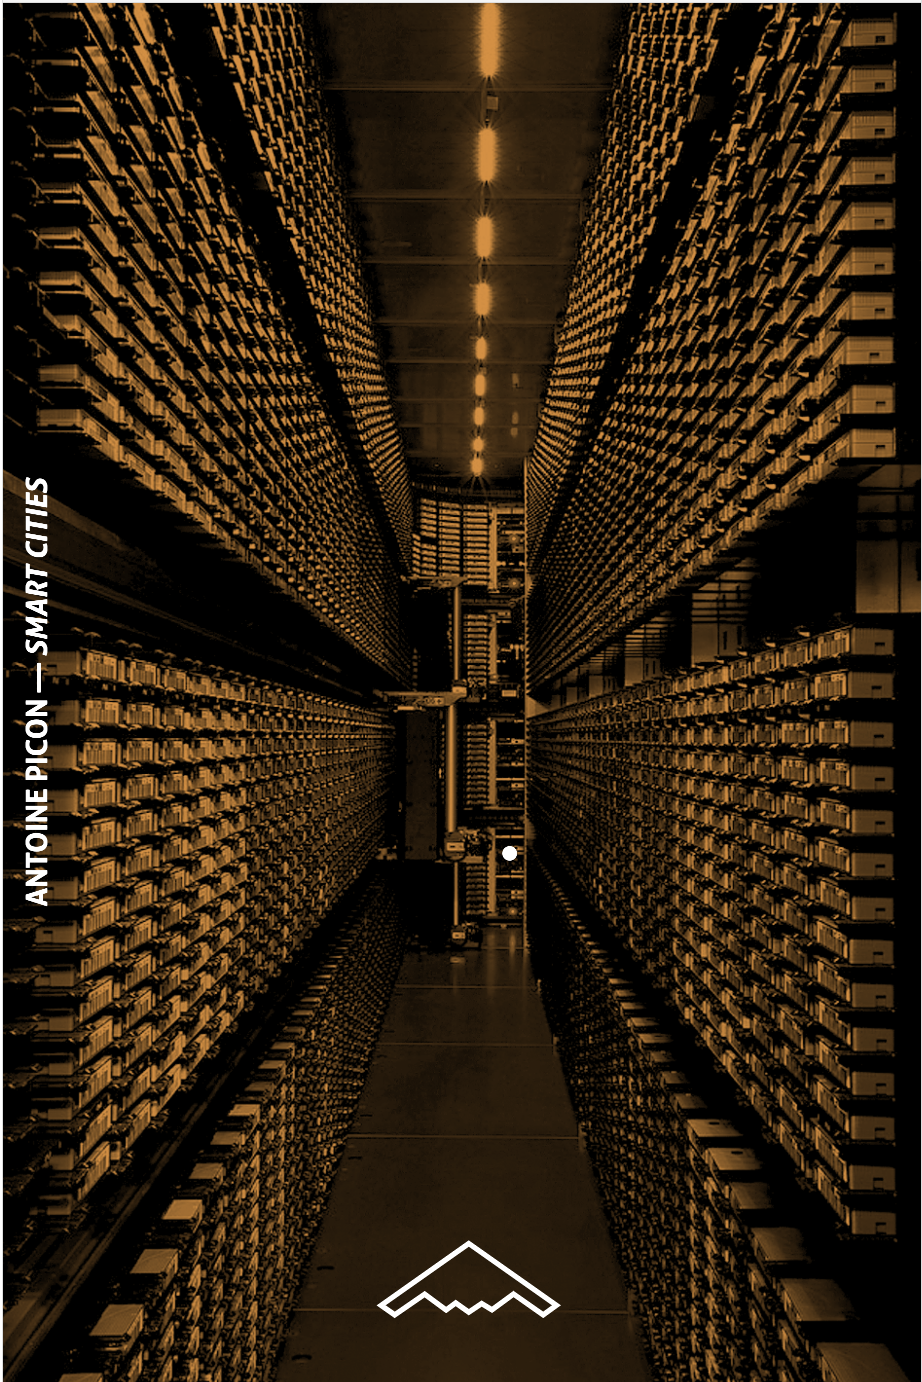
\includegraphics[height=0.4\textheight]{figures/picon_smartcities.png}


}


\sframe{Smart cities, digital twins and complexity}{

% - Arcaute, Elsa & Barthelemy, Marc & Batty, Michael & Caldarelli, Guido & Gershenson, Carlos & Helbing, Dirk & Moreno, Yamir & Ramasco, Jose Javier & Rozenblat, Céline & Sánchez, Angel. (2021). Future Cities: Why Digital Twins Need to Take Complexity Science on Board.   https://www.researchgate.net/publication/354446988_Future_Cities_Why_Digital_Twins_Need_to_Take_Complexity_Science_on_Board/link/6138bca0c76de21e319f536a/download

Urban planning and engineering start to build digital twins lacking underlying theories \cite{arcaute2021future}

\bigskip

$\rightarrow$ intrinsic obstacles in whole system modeling: chaos, algorithmic complexity, emergence

\medskip

$\rightarrow$ big data implies more theory, not less

\medskip

$\rightarrow$ integrate models in co-evolution with their socio-technical context \cite{commenges2013invention} 


}


\sframe{The real ``smart''? Long term urban analytics}{

% - urban analytics : policy Kandt, J., & Batty, M. (2021). Smart cities, big data and urban policy: Towards urban analytics for the long run. Cities, 109, 102992.

How can new urban data science approaches help for long-term policy-making? \cite{kandt2021smart}

\bigskip

$\rightarrow$ opposite temporalities of real-time high frequency analytics and long term slow urban change

\medskip

$\rightarrow$ role of subjectivity and political character of implementing such technologies

\medskip

$\rightarrow$ Propositions: generate hypothesis; more theory needed; complementarity with small data; search for long-term evidence; role of context; embrace alternative rationalities (urban perspectives \cite{pumain2020conclusion})


}


\sframe{Smart cities and blockchain: towards sustainability?}{

% sort of research question - narrative (to bring blockchain in?)

% field considered: "urban systems" - focus on infra/technical artifacts (social - governance aspects tackled by other pres, + link to digital twins/smart cities)

%\justify

Considering the field of \textbf{urban systems} and focusing on \textbf{infrastructure/technical artefacts} (social, governance, law aspects in other presentations):

\bigskip

$\rightarrow$ \textit{what is the place of blockchain in smart cities paradigms?}

\bigskip

$\rightarrow$ \textit{which place in sustainable transitions on the long-term?}


}



\section{Blockchain and smart cities}


% different fields - not comparable? (more in transport?)

\sframe{Blockchain and cities}{

%\cite{jabbar2022blockchain}
% all fields related to urban - smart cities: ~ supply chain, iot, energy management, transport, ~ governement (+voting?)

%\cite{shen2018blockchain}
% governance, eductaion-culture-sci-innov, health-safety, economy, transportation, energy, built environment: building resources, natural envt

Systematic reviews identify many fields related to cities and urban systems \cite{jabbar2022blockchain} \cite{shen2018blockchain}:

\medskip

\begin{itemize}
	\item \textbf{IOT, data management}
	\item \textbf{intelligent transport systems}
	\item \textbf{energy management}
	\item \textbf{built environment (building resources)}
	\item \textbf{supply chains}
	\item governance
	\item economy, finance
	\item education, culture, science, innovation
	\item health, safety	
	\item \ldots (list not exhaustive)
\end{itemize}



}

\sframe{Blockchain in transportation}{

% Jabbar, R., Dhib, E., ben Said, A., Krichen, M., Fetais, N., Zaidan, E., & Barkaoui, K. (2022). Blockchain Technology for Intelligent Transportation Systems: A Systematic Literature Review. IEEE Access.
In the case of transport systems \cite{jabbar2022blockchain}:

\bigskip

\begin{itemize}
	\item Services and transport system management
	\item Payments
	\item Security
	\item Data management
	\item Energy
	\item Comunication and networks
\end{itemize}


}

\sframe{Intelligent transport systems}{

% Balasubramaniam, A., Gul, M. J. J., Menon, V. G., & Paul, A. (2021). Blockchain for intelligent transport system. IETE Technical Review, 38(4), 438-449.
%-> data reduction and data integrity for legal purposes (digital proof in case of accidents by intelligent transport systems)
Accident data for autonomous vehicles: data reduction and integrity checking with blockchain (digital legal proofs) \cite{balasubramaniam2021blockchain}

\bigskip

\centering

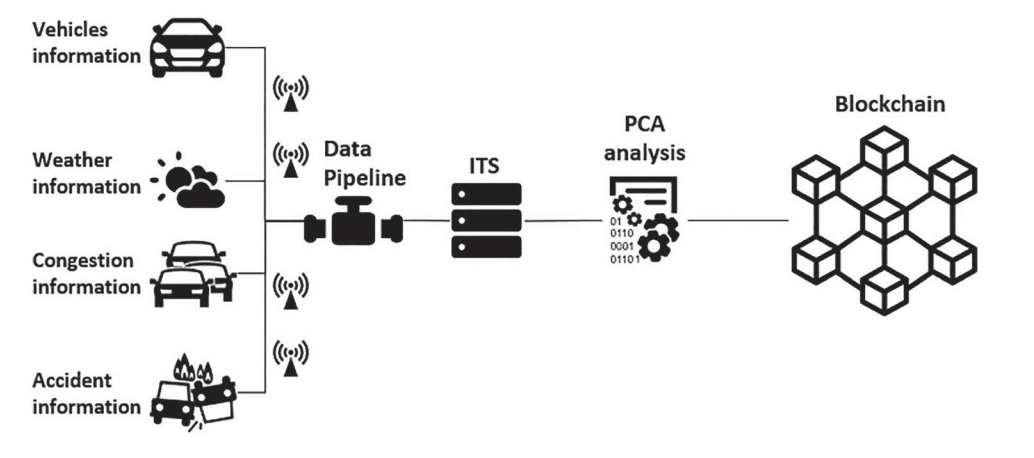
\includegraphics[height=0.57\textheight]{figures/blockchainAccident.png}


}

\sframe{Intelligent transport systems}{

% Kumar, R., Kumar, P., Tripathi, R., Gupta, G. P., Kumar, N., & Hassan, M. M. (2021). A privacy-preserving-based secure framework using blockchain-enabled deep-learning in cooperative intelligent transport system. IEEE Transactions on Intelligent Transportation Systems.
% -> autonomous vehicles communicates between themselves, road side units and traffic control centers : blockahin and deep learning algos to ensure: privacy and security. Smart contract to ensure data integrity
% rq: no detail of algo?
Autonomous vehicles communicate between themselves, with road side units and traffic control centres: blockchain and deep learning to ensure privacy and security \cite{kumar2021privacy}

\medskip

\centering

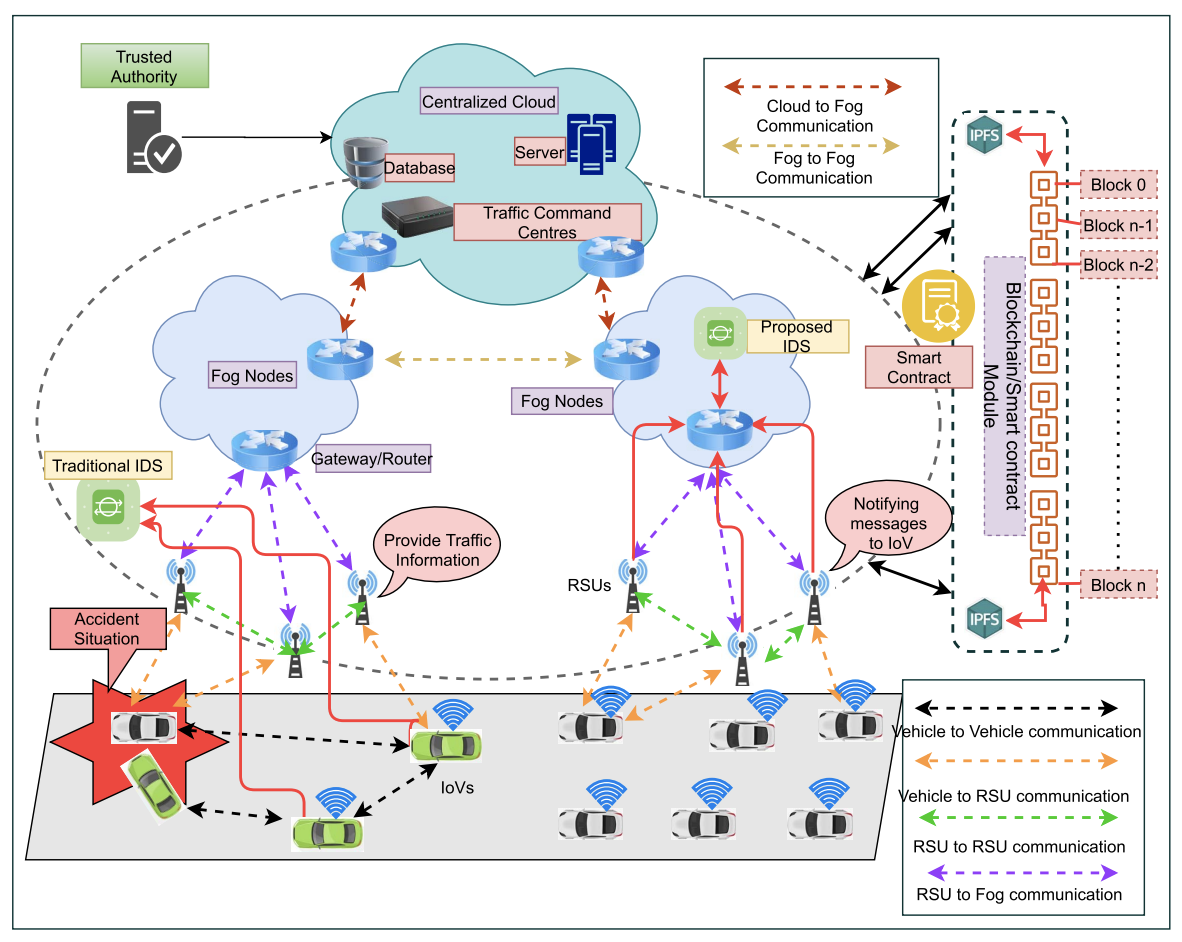
\includegraphics[height=0.7\textheight]{figures/auvcom.png}

}

%\sframe{}{
%\cite{singh2020convergence}
% - intelligent transport systems, vehicle rental
% - security issues?
%}





%\sframe{Privacy preservation}{

% -> in issues - developments
%Mezquita, Y., González-Briones, A., Casado-Vara, R., Wolf, P., Prieta, F. D. L., & Gil-González, A. B. (2021, April). Review of Privacy Preservation with Blockchain Technology in the Context of Smart Cities. In Sustainable Smart Cities and Territories International Conference (pp. 68-77). Springer, Cham.
%\cite{mezquita2021review}
%}

\sframe{Securing smart grids}{

% Kathrine, G. J. W., Javadi, B., Peter, J. D., & Palmer, G. M. (2021). An Intelligent Blockchain-Based Framework for Securing Smart Grid. In Industry 4.0 Interoperability, Analytics, Security, and Case Studies (pp. 81-94). CRC Press.
%\cite{kathrine2021intelligent} - not open!
% Mollah, M. B., Zhao, J., Niyato, D., Lam, K. Y., Zhang, X., Ghias, A. M., ... & Yang, L. (2020). Blockchain for future smart grid: A comprehensive survey. IEEE Internet of Things Journal, 8(1), 18-43. idem
% Alladi, T., Chamola, V., Rodrigues, J. J., & Kozlov, S. A. (2019). Blockchain in smart grids: A review on different use cases. Sensors, 19(22), 4862. bof
% Musleh, A. S., Yao, G., & Muyeen, S. M. (2019). Blockchain applications in smart grid–review and frameworks. Ieee Access, 7, 86746-86757.

Blockchain can be used in different components of heterogeneous smart grids \cite{musleh2019blockchain}

\bigskip

\centering

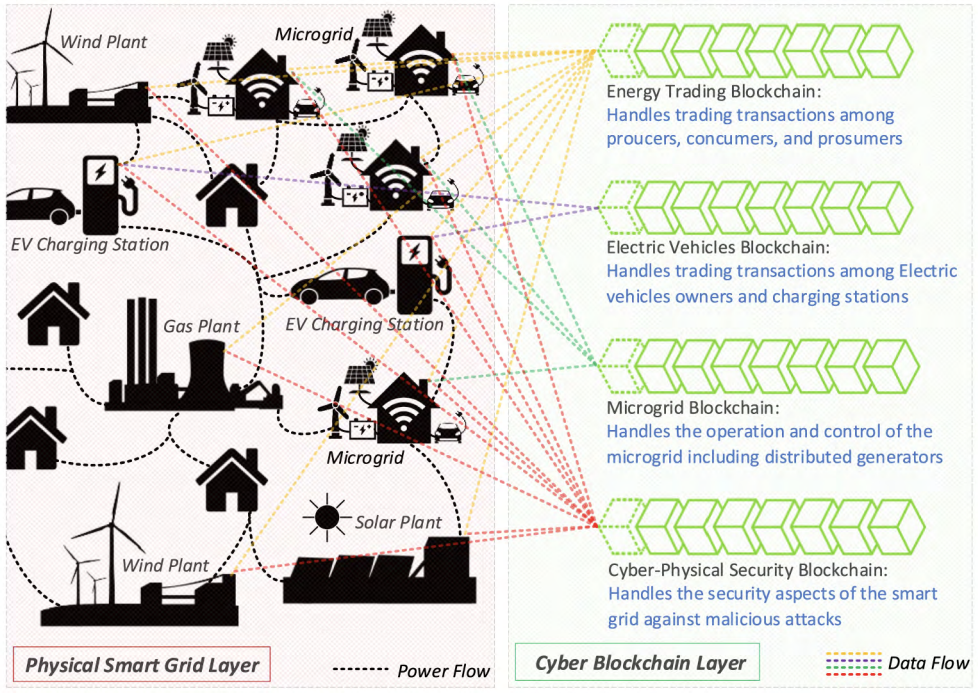
\includegraphics[height=0.75\textheight]{figures/smartgrid.png}

}

\sframe{Other urban applications}{

\begin{itemize}
	\item Tracking of waste collection \cite{laouar2019towards}
	\item Trading of development rights to contain urban sprawl \cite{allam2019potential}
	\item Management of building permits \cite{mora2019management}
	\item Public participatory GIS \cite{farnaghi2020blockchain}
	\item Logistics and deliveries \cite{tian2021blockchain}
	\item From cities to territories? agriculture \cite{bermeo2018blockchain}, ecology \cite{whitaker2020commodity}
	\item \ldots
\end{itemize}


}


%\sframe{From cities to territories?}{

% Agriculture
% exchange of products without the mediation of a third party; safety and reliability of transactions; high quality data; work with qualified users; process integrity; transparency and permanence of the system; simplified accounting system; efficient transactions
% smart contracts
% -~ cited above not orig paper (Russian author, crimea univ?) Bunchuk, N. A., Jallal, A. K., Dodonov, S. V., Dodonova, M. V., & Diatel, V. N. (2020). Perspectives of Blockchain Technology in the Development of the Agricultural Sector. Journal of Complementary Medicine Research, 11(1), 415-421.
%}


\sframe{Synthesis}{

% - main applications domains

\textbf{Main application domains: } transportation, energy, logistics

% - main issues
%     * from mezquita2021review: privacy: ML coupled with blockchain - not good enough yet for real implementation ; energy efficiency; proof of stake, proof of trust ; scalability ; incentives ; interoperability ; link with traditional governance structures?

\bigskip

\textbf{Main open issues for implementation} \cite{mezquita2021review}:

\begin{itemize}
	\item privacy preservation (coupling blockchain with machine learning)
	\item energy consumption: which blockchain algorithm?
	\item scalability, interoperability
	\item link with classical governance structures
\end{itemize}

\bigskip

% - perspectives
%     * from mezquita2021review: partocipatory sensing (smartphones as distributed sensors) ; distributed storage
%   

\textbf{Some perspectives} \cite{mezquita2021review}: participatory sensing (personal devices, IOT); distributed storage and computation; \ldots


}


\sframe{Discussion}{

% - cars: still doesnt solve congestion
% - actors implementing it / reproducibility / empowerment : social aspect of it?
% ? - link between scales - long term

\justify
\footnotesize

\vspace{-0.5cm}
\textit{From the geographer viewpoint:}

\bigskip

\textbf{On the use of blockchain: } which trade-offs between energy (emissions) gains and consumption? Other dimensions with trade-offs?


\bigskip

\textbf{On ICT infrastructures:} ``Smart'' systems may still intrinsically be non-sustainable: example of autonomous electric cars (even flying) remaining cars, with congestion, pollution, construction burden, \ldots

$\rightarrow$ smart (in the sense of elegant?) planning and design may be much more relevant: transit-oriented development and co-evolution \cite{raimbault2018caracterisation}, urban form and morphogenesis \cite{raimbault2014hybrid}, urban ecology \cite{raimbault2020spatial}, \ldots


\bigskip

\textbf{On stakeholders, social context, inequalities:} empowerment vs domination tools? \cite{leszczynski2022glitch}; implementation, reproducibility? opt-out / left-behinds?

\bigskip

\textbf{On the utility for long-term sustainable planning: } role of blockchain in operational digital twins with data integrity $\rightarrow$ strong coupling between scales remains an open issue in urban modeling \cite{raimbault2021strong}


}


\section{Conclusion}


\sframe{Conclusion}{

% answer RQ: ?
%  role of blockchain in smart cities - transfer of models towards governance - valo research? 

$\rightarrow$ many applications of blockchain for smart cities: at the state of research/prototype, mature technological transfer and valorisation remains to be made

\bigskip

$\rightarrow$ utility for long-term territorial policies for sustainable transitions? Complexity approaches and multi-scale modeling are necessary but still open and not operational

\bigskip

$\rightarrow$ more significant impact on economic, social, governance, law, digital, \ldots dimensions than on technical artefacts?



}



%%%%%%%%%%%%%%%%%%%%%
\begin{frame}[allowframebreaks]
\frametitle{References}
\bibliographystyle{apalike}
\bibliography{biblio}
\end{frame}
%%%%%%%%%%%%%%%%%%%%%%%%%%%%










\end{document}

